\documentclass{IOS-Book-Article}
\usepackage{graphicx}

\usepackage[square,numbers,sort]{natbib}

\usepackage{booktabs}
\usepackage{multirow}

\usepackage{color}
\usepackage{hyperref}
% http://colorschemedesigner.com/#4o42FfqublRMS
\definecolor{linkcolor}{RGB}{66, 54, 122}
\definecolor{citecolor}{RGB}{84, 141, 100}
\definecolor{urlcolor}{RGB}{168, 70, 67}
\hypersetup{
  colorlinks=true,
  linkcolor=linkcolor,
  citecolor=citecolor,
  urlcolor=urlcolor,
}
\def\UrlBreaks{\do\/\do-}

\usepackage{soul}
\definecolor{hlcolor}{RGB}{255, 221, 163}
\sethlcolor{hlcolor}
%\newcommand{\hl}[1]{#1}

\usepackage{mathptmx}

%\usepackage{times}
%\normalfont
\usepackage[T1]{fontenc}
%\usepackage[mtplusscr,mtbold]{mathtime}
%

\newcommand{\sn}[1]{\href{https://twitter.com/#1}{\texttt{@#1}}}


\newcommand{\zenodoBase}{https://zenodo.org/record/1299195}
\newcommand{\sfile}[1]{\href{\zenodoBase/files/#1}{#1}}

\begin{document}
\begin{frontmatter}              % The preamble begins here.

%\pretitle{Pretitle}
\title{Language Bias in a Multilingual Tweet Corpus}
%\runningtitle{LV2}
%\subtitle{Subtitle}

\hypersetup{pdfauthor={Dmitrijs Milajevs}}
\author[A]{\fnms{Dmitrijs} \snm{Milajevs}%
  \thanks{Corresponding Author: Dmitrijs Milajevs, Guest Researcher,
    100 Bureau Drive,
    Gaithersburg, MD 20899, USA%
    ;
    E-mail: dmitrijs.milajevs@nist.gov.}}
%\author[B]{\fnms{Second} \snm{Author}}
%and
%\author[B]{\fnms{Third} \snm{Author}


\runningauthor{D. Milajevs}
\address[A]{Guest Researcher at National Institute of Standards and Technology, Maryland, USA}
%\address[B]{Short Affiliation of Second Author and Third Author}

%\begin{abstract}
%
%\end{abstract}

\begin{keyword}
Corpus Linguistics \sep Latvian \sep Russian \sep English
\end{keyword}
\end{frontmatter}

\thispagestyle{empty}
\pagestyle{empty}

\section*{Introduction}

This paper presents a multilingual, location-anchored corpus of tweets from Latvia. The main challenge of collecting a socially representative corpus from this country is that several languages are used there: Latvian, the main communication language and the only official language in Latvia, Russian, the language of the largest minority in Latvia, and English.

%%%%%%%%%
% Problem
%%%%%%%%%
%There are several challenges of building a tweet collection that adequately represents language use in the country.
%
Building a monolingual Latvian collection could be done by harvesting tweets that contain indicative Latvian words, which are not present in other languages, similarly to how it is done for Dutch \cite{sang2013}. However, such an approach is not suitable for tweets in Russian and English, as these languages are widely used outside of Latvia.
%
For the same reason, a TREC-like collection building approach \cite{lin2017rts} of filtering the publicly available stream of tweets by language would not work.
%
A tweet collection based on a curated list of users \cite{SANVICENTE16.465,L14-1642} is effective, but extra care must be taken as a thematic bias might be introduced.
%
An alternative approach would be to retrieve only geo-located tweets \cite{coats_steven_2017,milajevs:2017:BUCC}. Such a collection would neither be biased linguistically because it is not based on a list of keywords, nor it would be biased thematically because it is not based on a list of users. The downside is that a large number of tweets are not geo-located, which makes retrieval incomplete.

%%%%%%%%
% Method
%%%%%%%%
To keep a balance between objectivity and completeness, this work applies a hybrid approach by combining a geo-location based collection procedure with following a curated list of users, which is based on the accounts of Latvian media outlets, politicians, government institutions and public figures.

Our base assumption is that geo-located tweets are a representative and unbiased sample of tweets from Latvia. Thus, an objective collection should exhibit similar properties as the geo-located one. The main property we study in this work is the language proportion. We hypothesize, that an objective extended collection should have similar language distribution as the initial.

To study the collection in more detail, we manually searched the collection for \hl{16} topics of interest.

%%%%%%%%%
% Results
%%%%%%%%%

The analysis shows that---despite our attempt---the extended collection is biased toward content in Latvian: proportionally there are more tweets in Latvian in the extended collection than in geo-located. We observe this phenomena not only at the ``global level'' (the whole collection), but also at the ``micro'' level (across the topics). \hl{In all but one topic, Latvian is more dominant than expected.}

%%%%%%%%%%%%%
% So, what...
%%%%%%%%%%%%%

Building an unbiased collection is difficult.  In our case the main reason of the introduced bias, might be that Russian and English content is less news-oriented and much more informal. In other words, while it is common to discuss current news in Latvian by engaging with the media, tweets in Russian and English tend to be personal and friend-oriented. Future work should verify whether this is actually the case.
% IMS is this a hypothesis you intend to test here?  Or is this future work?  Or what?

\section{Data collection}
\label{sec:data-collection}

Over the period from 15 April 2017 to \hl{8 May 2018} the initial set of \hl{1\,708\,236} tweets was collected from the \texttt{POST status/filter} endpoint of the Twitter Streaming API. Following \cite{milajevs:2017:BUCC}, the \texttt{locations} parameter was set to the bounding box of Riga, the capital of Latvia. It is small enought to fit into Twitter API restrictions and covers about 40\% of the popilation of Latvia.%\footnotemark{}
%
\footnotetext{The coordinates of the bounding box are \texttt{23.9325829, 56.8570671, 24.3247299, 57.0859184}.}
% IMS.2 according to http://worldpopulationreview.com/countries/latvia-population/, the population of Riga is less than half the total population of Latvia.  However, Twitter only allows bounding boxes for location to be so big, so you can't bound the whole country.

In addition to the location, 420 accounts were followed.\footnotemark{} The accounts are mostly Latvian (that is, coming from Latvia, but not necessary produce content in Latvian) news outlets, politicians, businesses, artists and sport clubs. We avoided following personal accounts to respect their privacy. We also avoided bootstrapping the list, as it might have introduced accounts that originate outside of Latvia, for example, \sn{BBC}. The whole list of screen names together with user IDs is available in the supplement file \sfile{lv.cfg}.

\footnotetext{In this paper, by ``following users'', we mean that their user IDs where passed to the Twitter API to collect tweets that they created, retweets of those tweets, or the tweets that are replies by other users to their tweets. Refer to the \href{https://developer.twitter.com/en/docs/tweets/filter-realtime/guides/basic-stream-parameters\#follow}{Twitter documentation} for a complete description. Keep in mind that this is different from the case when a user follows another user.}

% IMS how did you select those accounts? Can you describe them generically here?  (i.e. "Latvian news outlets, famous actors and politicians, and a selection of Eurovision finalists.")  You should make clear you hand picked them based on background knowledge or if this list was scraped from a public resource, since it reflects effort put into making the collection.

To comply with Twitter's terms of service, on \hl{8 May 2018}, the raw tweet data was redownloaded to get rid of deleted tweets. The tweets that originated a retweet were added to the collection. Also, we have noticed a large number of tweets that came from Sweden (probably because of the imprecise \texttt{locations} parameter value), so the tweets which location country code was \texttt{SE} were omitted. This resulted in \hl{1\,242\,943} tweets that formed the final collection presented here.\footnotemark{}

\footnotetext{The supplement files are available at Zenodo: \url{\zenodoBase}. Collected tweet IDs are available as \sfile{collected\_tweets.csv} and the final collection is available as \sfile{rehydrated\_tweets.csv}. The supplement files are licensed under a \href{https://creativecommons.org/publicdomain/zero/1.0/legalcode}{Creative Commons CCZero 1.0 License/Waiver}.}

\section{Twitter users}
\label{sec:global-analysis}

\begin{table}
  \centering
  \begin{tabular}{lrllrlrlrlrl}
\toprule
lang & total\_count & total\_share & tracked\_source\_share & \multicolumn{2}{l}{lv} & \multicolumn{2}{l}{ru} & \multicolumn{2}{l}{en} & other\_lang\_count & other\_lang\_share \\
{} & source\_lang\_count & source\_lang\_share & source\_lang\_count & source\_lang\_share & source\_lang\_count & \multicolumn{3}{l}{source\_lang\_share} \\
source\_pretty       &             &             &                      &                   &                   &                   &                   &                   &                   &                  &                  \\
\midrule
Twitter Web Client  &      465845 &       34.1\% &                52.4\% &            386342 &             82.9\% &             14718 &              3.2\% &             38715 &              8.3\% &            26070 &             5.6\% \\
Twitter for Android &      227534 &       16.7\% &                 8.3\% &            153578 &             67.5\% &             22351 &              9.8\% &             34632 &             15.2\% &            16973 &             7.5\% \\
Twitter for iPhone  &      205280 &       15.0\% &                14.0\% &            123388 &             60.1\% &             32796 &             16.0\% &             31829 &             15.5\% &            17267 &             8.4\% \\
TweetDeck           &      104345 &        7.6\% &                91.7\% &            102261 &             98.0\% &                75 &              0.1\% &              1470 &              1.4\% &              539 &             0.5\% \\
TVNET Login         &       57733 &        4.2\% &                96.7\% &             26231 &             45.4\% &             30826 &             53.4\% &                23 &              0.0\% &              653 &             1.1\% \\
dlvr.it             &       45337 &        3.3\% &                98.4\% &             44806 &             98.8\% &               134 &              0.3\% &               129 &              0.3\% &              268 &             0.6\% \\
Facebook            &       36327 &        2.7\% &                95.1\% &             13741 &             37.8\% &             20833 &             57.3\% &               450 &              1.2\% &             1303 &             3.6\% \\
Foursquare          &       30708 &        2.3\% &                 0.0\% &             24300 &             79.1\% &               220 &              0.7\% &              1881 &              6.1\% &             4307 &            14.0\% \\
Instagram           &       24654 &        1.8\% &                 1.7\% &              8801 &             35.7\% &              2450 &              9.9\% &              8164 &             33.1\% &             5239 &            21.3\% \\
SKATIES             &       22798 &        1.7\% &                98.0\% &             22782 &             99.9\% &                 0 &                 0 &                 0 &                 0 &               16 &             0.1\% \\
\bottomrule
\end{tabular}
  
  \caption{Global statistics.}
\end{table}

On average, about \hl{3\,200} tweets were collected per day, which is more than 1\,500 by the geo-location based technique in \cite{milajevs:2017:BUCC}. Most of the tweets came from the official Twitter clients for Web, Android or iPhone. Together these clients contributed more than 60\% of all collected tweets, refer to Table~\ref{tab:source_counts} for more details.

The twitter web client is used by both the general public and media companies. The top 5 of most active accounts consists only of followed Latvian media accounts: \sn{DienaLV} (a newspaper), \sn{LA\_lv} (another newspaper), \sn{JaunsLV} (a media portal), \sn{TV3\_Play} (a TV channel), and \sn{dblv} (a newspaper).

%Notably, for mobile clients, the majority of tweets comes from \hl{the general public}, because they are either geo-located or mention a followed account.
The proportion of tweets coming from followed accounts is lower for Android \hl{(8.4\%)} than for iPhone \hl{(13.8\%)}. The difference can be explained by the insight, that all top 5 Android users are personal accounts, while for iPhone there are only 2 personal accounts in the top 5. \sn{TV3zinas} (a news account of a TV channel) tweets the most from iPhone. \sn{Lattelecom} (a telecommunication company) is the second most active iPhone user. \sn{AstrologiLv} writes about astrology and is the fourth most active iPhone user. All three accounts tweet exclusively in Latvian and were followed during corpus collection.

%Client applications that produce tweets mostly from tracked accounts are used by the media. 
% IMS I don't understand the previous sentence
For the TweetDeck, TVNET Login, dlvr.it and SKATIES client applications the top 5 users are followed media accounts that write dominantly in Latvian. The exceptions are a business account \sn{Kompresori} that was not followed and tweets in three languages: Latvian, Russian and English, \sn{RusApollo} and \sn{TVNET\_rus} who tweet identical content exclusively in Russian, and \sn{SejasLV}, an exclusively Latvian account writing about celebrities, which was not followed.

% IMS terminology jumble. You are tracking, and also other users are tracking, and you selected users who were tracking (well, actually, probably retweeting) tweets from accounts you were tracking already.  You want this section to read like a recipe for your reader who wants to duplicate your effort in Swahili or whatever.

TweetDeck is used by \sn{DelfiLV} (a major media portal), \sn{LV\_Portals}, (the official government gazette), \sn{lsmlv} (a publicly funded radio and television organization (LSM)), \sn{ltvzinas} (the news account of Latvian Television) \sn{RietumuRadio} (a radio station). 

TVNET is a media company that controls several media portals. The most active accounts that use their application are \sn{TVnet\_portals}, \sn{RusApollo}, \sn{TVnet\_rus}, \sn{SportsTVNET}, and \sn{SejasLV}. As mentioned above, \sn{RusApollo} and \sn{TVnet\_rus} post identical messages.

The tweet delivery service \texttt{dlvr.it} is used by the newspaper \sn{nralv} and their sport portal \sn{Sportacentrs}, the photo account of the national news agency (LETA) \sn{letafoto}, \sn{Kompresori} and the sport account of Latvian Television \sn{ltvsports}.

SKATIES delivers video content from several sources. The most active accounts are \sn{skatieslatvija}, \sn{lnt\_lv}, \sn{tv3lv}, \sn{BezTabuTV3} and \sn{TV3Zinas}.

Some tweets are crossposts from other social media networks. Facebook content mostly comes from the followed media accounts. The top 5 most active users are: \sn{mixnews\_lv} (the Russian edition of the Mixnews.lv media portal), \sn{Otkrito} (the Russian edition of \sn{JaunsLV}), \sn{labdienlv}, \sn{ekonimikalv} and \sn{nozare} (all three belong to the same media company and tweet in Latvian).
%The fact that Russian accounts are not active among other clients might suggest that Russian content is not spread initially via Twitter, but is cross-posted from Facebook.
% IMS but you said you were tracking Facebook.  I think you mean that you can only track FB when the content is also posted to Twitter, but not otherwise.

%The content that is crossposted from Foursquare and Instagram is created by the accounts that are not followed.
% IMS.2 same comment as above... when you say "comes from" you mean crossposted content, right?  It's confusing because you also say "comes from" to mean the organization authoring the content.

%There is a clear pattern that mobile clients are used by personal accounts, while media companies set up a special solution to deliver tweets, probably, integrating it with their content delivery systems or simply using a web client from an office machine.

% IMS I wonder if a flow diagram would illustrate the paths this information takes before it gets on Twitter.

\section{Language}
\label{sec:language}

\begin{figure}
\centering

\caption{Tweet volume by day per language averaged over a rolling window of 7 days.}

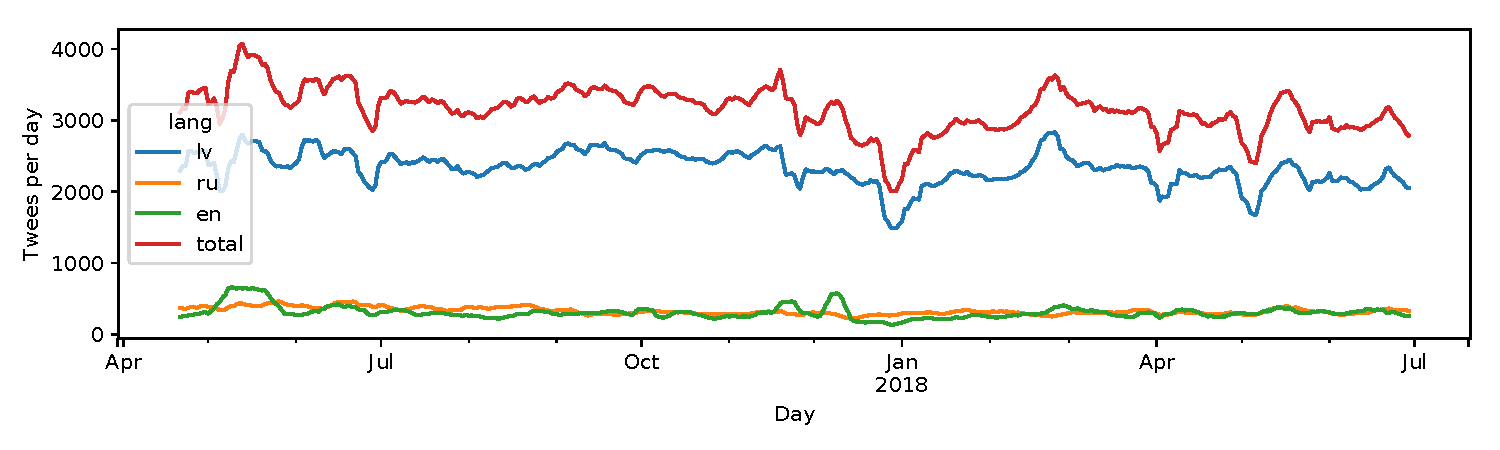
\includegraphics[width=\textwidth]{supplement/rehydrated_tweets_count_by_day.pdf}

\label{fig:rehydrated-tweets-count-by-day}
\end{figure}

%%% Local Variables:
%%% mode: latex
%%% TeX-master: "../paper.tex"
%%% End:

Latvian is the dominant language: \hl{917\,259 (73.8\%)} tweets are written in it.\footnotemark{} There are \hl{130\,825 (10.5\%)} tweets in Russian, \hl{122\,490 (9.9\%)} in English and \hl{72\,369\, (6.2\%)} in other languages. This distribution is very different from a geo-located method used in \cite{milajevs:2017:BUCC}, where the distribution is 44.5\% Latvian, 33.9\% Russian and 20.7\% English. Figure~\ref{fig:rehydrated-tweets-count-by-day} shows the tweet volume over time.

The tweets were written by \hl{41\,170} users. We refer to a user who produced at least 50 tweets as an \textit{active user}. There are \hl{2\,766} (\hl{6.7\%}) active users who produced \hl{1,196,558} (\hl{86.6\%}) tweets in total.

Among active users, \hl{789} are monoligual. Exclusively in Latvian write \hl{631} (\hl{80.0\%}), in Russian \hl{40} (\hl{5.1\%}) and in English \hl{118} (\hl{15.0\%}).

The Language uniformity score is defined in \cite{milajevs:2017:BUCC}. It is the normalized number of tweets in the most frequent language. Figure~\ref{fig:uniformity_score} compares the language uniformity scores of active users in this work and in \cite{milajevs:2017:BUCC}. Apart of the higher number of active users in this work (which is expected, as the corpus covers a longer period), the currently presented corpus has more active users with the language uniformity score about 0.5. Even though the majority is mostly monoligual, this work captured more (at least) bilingual users.

\begin{figure}
  \centering
  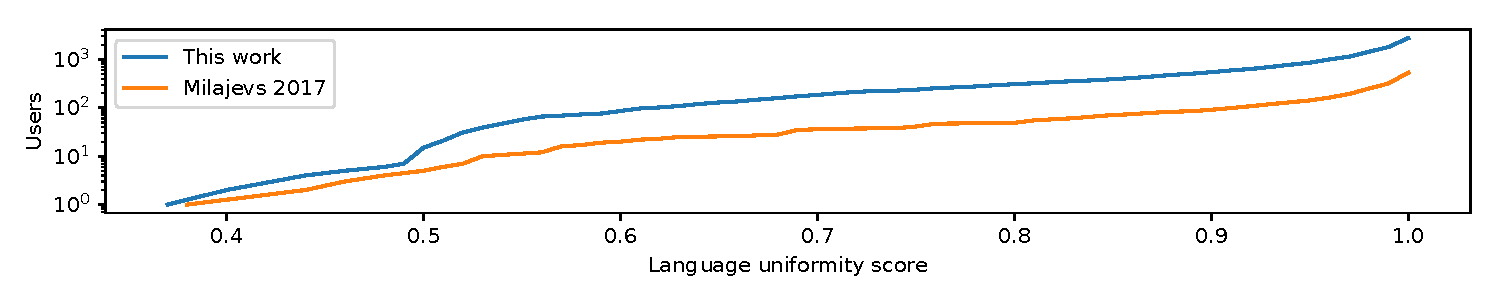
\includegraphics[width=\textwidth]{supplement/uniformity_score.pdf}
  \caption{Accumulative number of users by the uniformity score. Note the logarithmic Y-scale. Milajevs 2017 is \cite{milajevs:2017:BUCC}.}
  \label{fig:uniformity_score}
\end{figure}

\footnotetext{Twitter labels tweets with the language they are written in.}

%Latvian dominates almost in every client application (see Table~\ref{tab:source_counts}).
%Tweets coming from Foursquare are labeled as Latvian in \hl{78.4\%} cases.
% , that might be due to Latvian location names.
%
%More than half tweets that come from TVNET are in Russian. Its share is \hl{52.8\%} while Latvian's is \hl{46.1\%}.
%
%Same goes for tweets that come from Facebook, where the two most active users are the Russian edision of media portals (\sn{mixnews\_lv} and \sn{Otkrito}).
%
%A lot of English content is coming form Instagram (\hl{36.1\%}), that might be due to the dominance of hashtags over other text. Also, there are many tweets labeled as written in other languages that come from Foursquare and Instagram. As Instagram posts are more likely to contain hashtags and Foursqure tweets contain location names, tweets should not be assigned a single language label, but instead be labeled as written in several languages.

% IMS the point of the paper is that you believe this is a more representative sample than would be obtained by simpler methods.  Why do you believe it?  Is the hypothesis falsifiable?

% IMS is there code-switching?  How are you deciding that a tweet is in one language vs another?

\section{Topics}
\label{sec:topics}

To investigate the collection further, \hl{16} topics of interests were defined. The collection was manually searched using keywords to get relevant tweets. To compensate rich morphology in Latvian and Russian, keywords were manually stemmed. For example, \texttt{hokej} was used instead of Latvian \textit{hokejs} to search for the tweets about ice hockey. 

The topics are:\footnotemark{}
\footnotetext{The topic file is available as \sfile{topics.json.txt}.}
\begin{itemize}
\item \texttt{LV016:} \textbf{Latvia 100} \ The Centennial Celebration of the Republic of Latvia.
\item \texttt{LV005:} \textbf{Ice hockey} \ Ice hockey.
\item \texttt{LV003:} \textbf{Refugees} \ Refugee crisis in Europe, attitude to immigration and immigrants.
\item \texttt{LV009:} \textbf{Brexit} \ Withdrawal of the United Kingdom from the European Union known as Brexit.
\item \texttt{LV002:} \textbf{The Chronicles of Melanie} \ Mel\=anijas Hronika (The Chronicles of Melanie) is a Latvian movie that was selected for the Foreign-Language Category for Oscars.
\item \texttt{LV004:} \textbf{Blizzard of Souls} \ A Latvian movie Dv\=ese\c{l}u Putenis (Blizzard of Souls) that is in production by the time of writing.
\item \texttt{LV001:} \textbf{Winter} \ Winter, snow and cold weather.
\item \texttt{LV015:} \textbf{May 4} \ The Restoration of Independence Day.
\item \texttt{LV011:} \textbf{May 8-9} \ Remembrance of the end of Word War II (May 8). It is also honored as the Victory Day on May 9. The Europe Day is observed on May 9. Tweets about any of the three events are relevant.
\item \texttt{LV010:} \textbf{Midsummer} \ Midsummer celebration on June 23-24.
\item \texttt{LV014:} \textbf{November 11} \ A memorial day for soldiers who fought for the independence of Latvia.
\item \texttt{LV013:} \textbf{November 18} \ Proclamation Day of the Republic of Latvia.
\item \texttt{LV006:} \textbf{Christmas} \ Christmas.
\item \texttt{LV007:} \textbf{New Year} \ New Year.
\item \texttt{LV008:} \textbf{Olympics} \ The Olympic games and the Latvian team.
\item \texttt{LV012:} \textbf{March 16} \ Remembrance Day of the Latvian legionnaires.\footnotemark{}
\end{itemize}

\footnotetext{For more information about the event, refer to \url{http://www.mfa.gov.lv/en/policy/information-on-the-history-of-latvia/the-latvian-government-s-position-on-16-march-events}.}

% IMS I note your topics are titled either in Latvian or English.  Is that intentional?  Does it reflect a goal of boosting content from those languages?  Bigger question: why these topics?  More esoteric question: what value are the topics adding to your collection?  How many topics should you have?
Topics exhibit various temporal patterns, refer to Figure~\ref{fig:topic_timeline}. The volume of tweets is constant for long-lasting news stories such as the centennial celebration, the refugee crisis, Brexit and ice hockey.
%
During the Ice Hockey World Championship the volume of hockey related tweets increases. Similarly, event-based topics---such as Christmas, New Year and Olympics---are the most active during corresponding events, the volume of tweets builds up as an event approaches.

In case of Christmas, we see unexpected activity in March which is due to the discussion of making the Orthodox Christmas a public holiday in Parliament. This topic exhibits some cultural differences and language use. Tweets in Latvian peak during Advent and Christmas in December, tweets in Russian reach maximum both in December and early January when Orthodox Christmas are celebrated. It is worth noting that during the discussion whether Orthodox Christmas should be a public holiday, it sometimes was referred as ``Russian Christmas.'' In spring, November 11 became a public holiday, thus a spike in activity.  Other event-related topics (May 4, May 8-9, etc.) behave similarly: their activity peaks during the event.

Topics about movies are the smallest volume-wise. For a movie that was shown at several international festivals, we see multilingual content, while tweets about a movie that is still in production are solely monolingual.

The topic about Winter is an example of a seasonal topic, which is mostly about the weather, the pictures of snow and driving conditions.

Table~\ref{tab:topic_lang_counts} shows the total number of tweets per topic and language share for Latvian, Russian and English. For most topics the share of Latvian tweets is higher than on average in the collection (Section~\ref{sec:language}). For Russian and English these numbers are generally lower than the global average.

The most notable exceptions (share of Russian tweets greater than \hl{10\%}) are Russian tweets about New Year and May 8-9. The topic about Winter comes close for Russian (\hl{9.6\%}) with respect to the expected average, but is low for English tweets. Interestingly, for the international news topics, there is proportionally more English content about Brexit than about refugees.

\begin{table}
  \centering

  \begin{tabular}{llrrrr}
\toprule
TopicID  & Title &  Latvian & Russian & English &  Tweets \\
\midrule
LV001    &  85.9\% &  9.6\% &  4.4\% &   9721 \\
LV002    &  88.8\% &  0.9\% & 10.2\% &    215 \\
LV003    &  88.9\% &  6.7\% &  4.4\% &   2968 \\
LV004    & 100.0\% &  0.0\% &  0.0\% &    225 \\
LV005    &  94.5\% &  2.4\% &  3.1\% &  26838 \\
LV006    &  86.5\% &  4.6\% &  8.9\% &   3632 \\
LV007    &  77.2\% & 14.4\% &  8.5\% &   1463 \\
LV008    &  95.3\% &  4.0\% &  0.7\% &   7518 \\
LV009    &  84.7\% &  4.9\% & 10.4\% &   2062 \\
LV010    &  85.5\% & 11.6\% &  2.9\% &   1290 \\
LV011    &  84.0\% & 13.9\% &  2.2\% &   1154 \\
LV012    &  94.6\% &  3.4\% &  2.0\% &    496 \\
LV013    &  94.0\% &  6.0\% &  0.0\% &    783 \\
LV014    &  89.1\% &  1.8\% &  9.1\% &   1022 \\
LV015    &  98.1\% &  1.9\% &  0.0\% &   1200 \\
LV016    &  86.5\% &  1.4\% & 12.1\% &   6804 \\
\bottomrule
\end{tabular}

  
  \caption{Number of relevant tweets per topic and language distribution.}
  \label{tab:topic_lang_counts}
\end{table}
\begin{figure}
  \centering
  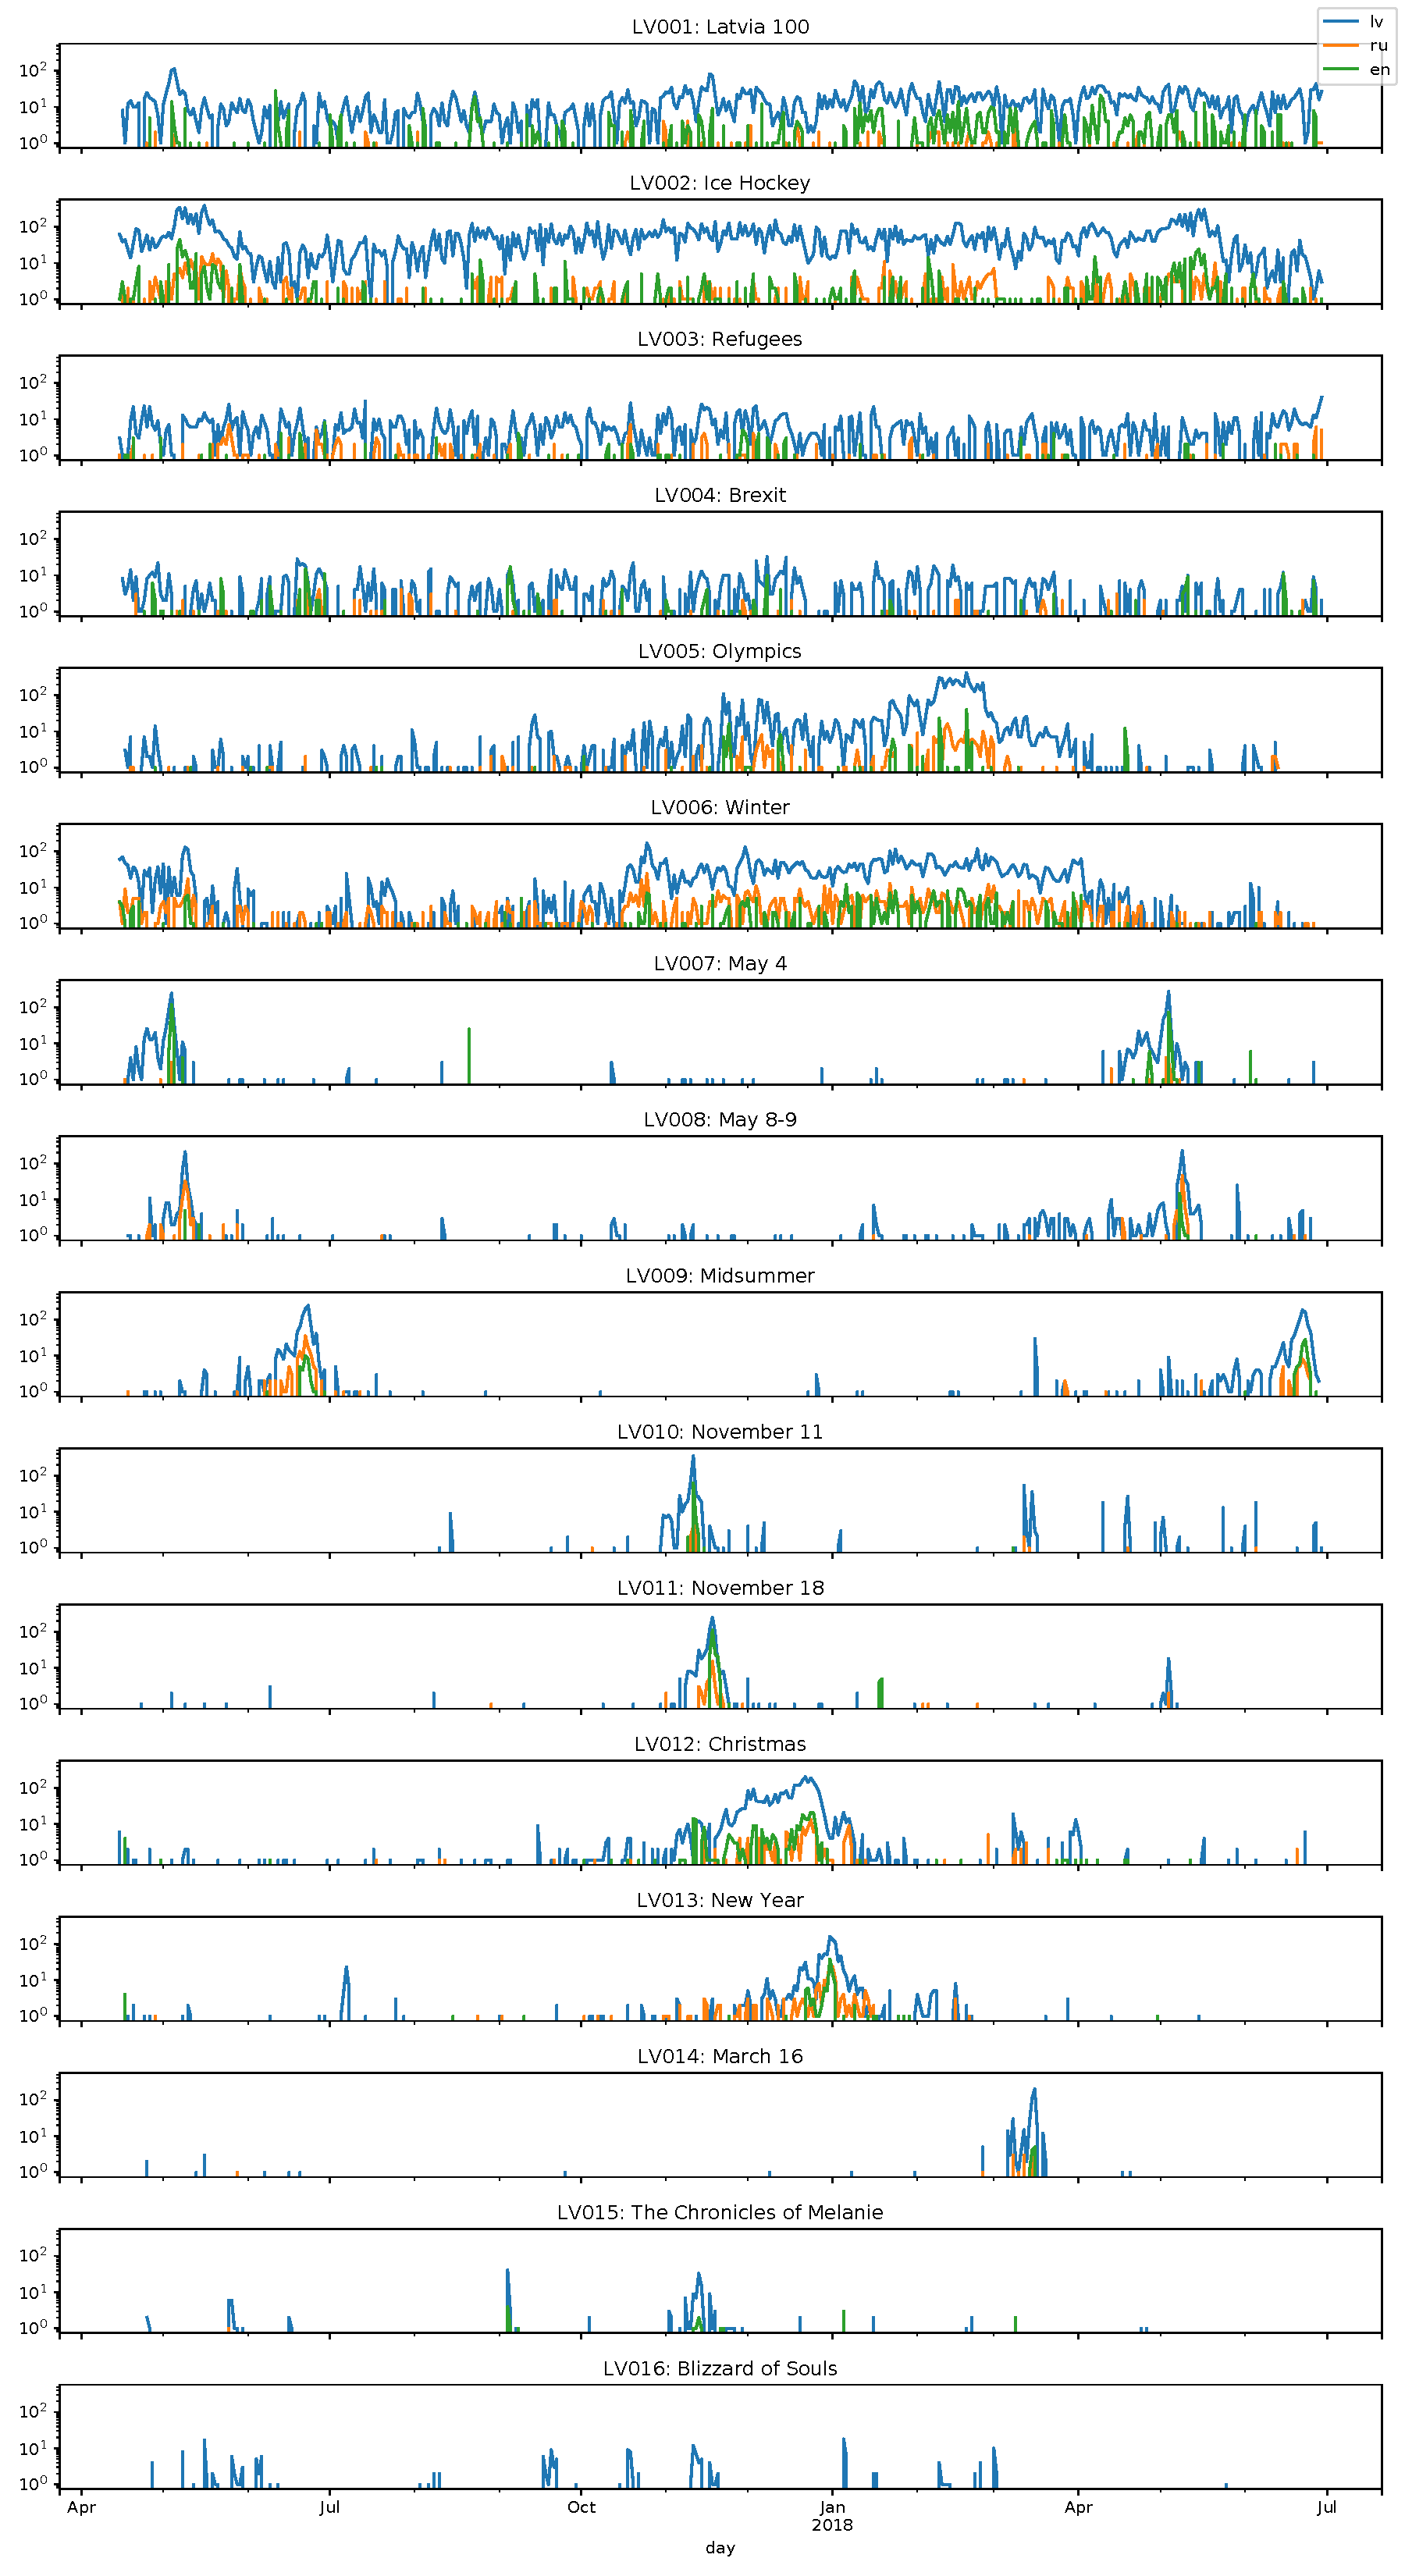
\includegraphics[width=\textwidth]{supplement/topic_timeline.pdf}
  \caption{Topic timeline. Note the logarithmic Y-scale, which is the number of tweets.}
  \label{fig:topic_timeline}
\end{figure}

\section{Conclusion and future work}
\label{sec:conclusion}

% IMS The conclusion does not address any of the questions raised in the abstract/introduction.

This paper presented a multilingual tweet collection with some analysis of users, language use and content. The analysis revealed differences in language use between the geo-located collection, global collection and topical sub-collections.

However, the question of whether the collection is any good remains open. It would be easy to test its extrinsic properties, for example, whether it leads to improvements in a language identification system when used as training data. But does not reveal its intrinsic properties. However, we believe the presented dataset might be useful across different studies.

As the corpus includes tweets of major media outlets and public figures, together with retweets and replies, it might be used to analyze public engagement.

From the sociolinguistic perspective, instead of avoiding bias, one could study what linguistic environment the tweets represent. What are the factors determining the language, contents and stance of a tweet. How do these factors interact? Who are the people writing those tweets?

Collection exploration trough keyword search showed that there is a lot of content on various topics and it should be feasible to run a shared retrieval task to evaluate retrieval systems and study what factors determine relevance.

%The challenges of building representative and complete tweet collection are:
%\begin{itemize}
%\item How the content of users who do not engage with media accounts (newspapers, radio stations, etc.~\ldots) might be collected respecting their privacy and not introducing bias into the collection?
%\item How to get hints of what topics are more popular among ``minorities''? What are tweets in Russian and English are about?
%\item Some tweets are multilingual. How can code-switching be detected reliably?
%\end{itemize}


\bibliographystyle{unsrtnat}
\bibliography{references,dmilajevs_publications}

\end{document}
